\documentclass[12pt,a4paper,catalan]{article}
\usepackage[utf8]{inputenc}
\usepackage[catalan]{babel}
\usepackage{amsmath}
\usepackage{amsfonts}
\usepackage{amssymb}
\usepackage{graphicx}
\usepackage{float}
\usepackage{framed}
\usepackage{url}
\graphicspath{{images/}}
\author{Marc Ferrer Fontirroig}
\title{Rehabilitació complementaria basada en videojocs utilitzant Leap Motion}
\begin{document}
	\begin{center}
		
\includegraphics{uib-logo.jpg}
	\end{center}
	\begin{center}
		\textbf{ESCOLA POLITÈCNICA SUPERIOR}\\
		\textbf{UNIVERSITAT DE LES ILLES BALEARS}\\
		\vspace{2em}
		\textbf{PROJECTE FINAL DE CARRERA}\\
		\vspace{1.5em}
		\textbf{ESTUDIS:}
		\begin{framed}
			\textbf{ENGINERIA INFORMÀTICA}
		\end{framed}
		\textbf{TÍTOL}
		\begin{framed}
			\textbf{REHABILITACIÓ COMPLEMETARIA BASADA EN VIDEJOCS UTILITZANT LEAP MOTION}
		\end{framed}
		\vspace{1.7em}
	\end{center}
	\begin{flushright}
		\textbf{Autor:} Marc Ferrer Fontirroig\\
		\textbf{Directora:} Cristina Manresa Yee\\
	\end{flushright}
	\textbf{Data:} Juny 2017
	\newpage
	\tableofcontents
	\newpage
	\section{Introducció}
	\subsection{Motivació}
	\subsection{Objectius}
	L’objectiu principal d’aquest projecte fi de carrera, és realitzar una prova de concepte d’exercicis de rehabilitació de lesions de les articulacions de la mà (canell i dits) utilitzant interfícies basades en visió comercials.
	
	La utilització d’exercicis basats en videojocs, aporta un context motivacional extra que pot ajudar a augmentar la participació dels usuaris en la seva teràpia de rehabilitació, tant en temps invertit, com en quant a l’atenció a aquests exercicis. Això és un aspecte fonamental per a l’èxit de la rehabilitació.
	
	La teràpia remota basa da en videojocs presenta un desavantatge, i és la falta de supervisió per part del responsable de la rehabilitació, típicament un fiseoterapeuta.
	
	Per tal de suplir aquest desavantatge un dels objectius d’aquesta prova de concepte és que les aplicacions és que el responsable de la teràpia sigui capaç de veure una reproducció dels moviments realitzats per l’usuari. D’aquesta manera es pot fer un seguiment de l’evolució de l’usuari més de manera més ràpida. De la mateixa manera el responsable de la teràpia és capaç de detectar possibles errors en la realització dels exercicis de rehabilitació, que d’una altra manera podrien tenir un efecte perjudicial per l’usuari, i aquests es poden corregir de manera gairebé immediata.
	
	En concret, es pretén utilitzar el controlador Leap Motion. El Leap Motion, és un dispositiu capaç de detectar i capturar les dades de les mans i els dits dins el seu camp de visió, sense necessitat d’utilització de cap tipus de marca de referència. Tot i que no està específicament dissenyat per a rehabilitació, el seu preu reduït i les seves dimensions en comparació a altres dispositius de visió, fan que aquest sigui un dispositiu idoni per els tipus d’exercicis proposats.
	\section{Treballs relacionats}
	\section{Anàlisi i disseny}
	\subsection{Introducció}
	\indent Dins aquest apartat s’analitza i descriu quin ha estat el sistema desenvolupat per tal de satisfer els objectius plantejats anteriorment.
	
	En primer lloc es presenta una descripció de l’arquitectura i les caracterís-tiques del controlador Leap Motion.
	
	Posteriorment es fa una anàlisi de requisits del sistema a desenvoluapar tant des del punt de vista fucional com tecnològic, la qual cosa permet tenir una descripció detallada del sistema.
	
	Com a darrera secció es descriu el disseny de l’aplicació amb tots els seus subsistemes i els diferents jocs desenvolupats, així com els seus detalls d’implementació.
	
	\subsection{Leap motion}
	El Leap motion és un dispositiu petit dispositiu que es connecta mitjançant USB i que és capaç de capturar els moviments de mans i dits, així com gestos i com petits objectes com llapis. Per fer-ho utilitza dues càmeres i tres LEDs infrarojos, el dispositiu és capaç de capturar les dades de les mans fins a una distància d’uns 60cm [1].
	
	Les dades capturades per aquestes càmeres són enviades per USB al ordinador al qual es connecta el controlador Leap, on el software de Leap Motion, que s’executa com un servei, s’encarrega de processar-les i deixar-les disponibles per a que puguin ser obtingudes mitjançant APIs.
	
	\subsubsection{Arquitectura del Leap Motion}
	El Leap Motion és capaç de funcionar en múltiples sistemes operatius i les seves dades poden ser obtingudes de dues formes; mitjançant una interfície nativa o a través d’un servidor de Web socket. D’aquesta manera, les possibilitats per als desenvolupadors són molt diverses i inclouen molts dels llenguatges de programació més utilitzants actualment [2].
	
	\paragraph{Interfície nativa}
	La interfície nativa es proporciona a través d’una llibreria que connecta el servei del Leap Motion. Aquest servei després proveeix les dades de seguiment obtingudes a les apliacions desenvolupades. La llibreria es pot utilitzar directament en el cas d’aplicacions desenvolupades amb C++ i Objective C, o es poden utilitzar una de les APIs per Java, C\# o Python [2].
	
	\begin{figure}[H]
		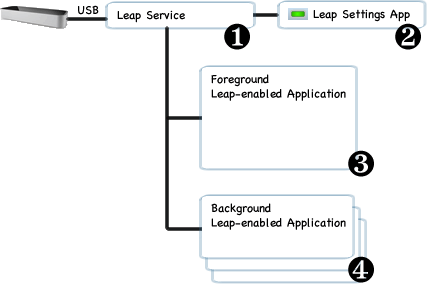
\includegraphics[width=\textwidth,keepaspectratio]{native-interface.png}
		\centering
		\caption{Esquema d'aplicacions utilitzant la interfície nativa.}
	\end{figure}
	\begin{enumerate}
		\item El servei de Leap Motion rep les dades del controlador a través d’una connexió USB, processa les dades rebudes i les envia a les aplicacions. Per defecte el servei només envia informació a les aplicacions en primer pla, però les aplicacions poden demanar rebre dades també en segon pla.
		\item L’aplicació de Leap Motion és independent del servei i permet als usuaris configurar la seva instal·lació de Leap Motion.
		\item Una aplicació en primer pla rep dades de seguiment del servei de Leap Motion.
		\item Quan una aplicació perd el focus del sistema operatiu, el servei de Leap Motion deixa d’enviar-li dades. Les aplicacions dissenyades per funcionar en segon pla poden demanar al servei que els proveeixi dades de seguiment fins i tot en segon pla.
	\end{enumerate}
	
	\paragraph{Interfície web socket}
	El servei de Leap Motion executa un servidor de web socket local en el domini local (localhost) a través del port 6437. Aquesta interfície de web socket proveeis dades de seguiment en format JSON. Després un client JavaScript desenvolupat per la mateix empresa de Leap Motion, s’encarrega de capturar aquestes dades i presentar-les com a objectes de JavaScript estàndard.
	
	\begin{figure}[H]
		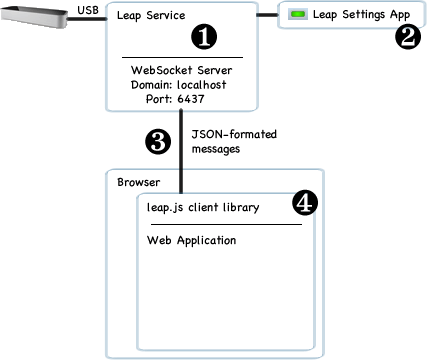
\includegraphics[width=\textwidth,keepaspectratio]{websocket-interface.png}
		\centering
		\caption{Esquema d'aplicacions utilitzant la interfície de web socket.}
	\end{figure}
	
	\begin{enumerate}
		\item El servei de Leap Motion proveeix un servidor de web socket a través de la direcció http://127.0.0.1:6437.
		\item L’apliació de configuració del Leap Motion permet habilitar o deshabilitar el servidor de web socket.
		\item El servidor envia les dades de seguiment en format JSON. Les aplicacions també poden enviar missatges de configuració al servidor.
		\item La mateixa empresa de Leap Motion ens proveeix d’una llibreria JavaScript que pot ser utilitzada per les aplicacions web per accedir a les dades de seguiment del Leap Motion.
	\end{enumerate}
	
	Aquesta interficie està dissenyada per ser utilitzada per aplicacions web, tot i que qualsevol aplicació pot establir una connexió amb el servidor de web socket. Aquest servidor segueix l’estàndard de web socket RFC6455

	\subsection{Requeriments}
	Tot i l'objectiu principal del projecte és realitzar una prova de concepte per confirmar que és possible utilitzar el controlador Leap Motion per complementar i monitoritzar teràpies de rehabilitació, és important establir una sèrie de requeriments tècnics i funcionals del projecte per tal de definir bé el seu abast.
	\subsubsection*{Requeriments d'usuari}
	\begin{description}
		\item [RU1] Un usuari ha de poder seleccionar un exercici a realitzar d’una llista.
		\item [RU2] Un usuari ha de poder realitzar exercicis d’extensió del canell.
		\item [RU3] Un usuari ha de poder realitzar exercicis d’abducció i adducció del canell.
		\item [RU4] Un usuari ha de poder realitzar exercicis d’abducció i adducció dels dits.
		\item [RU5] Un Responsable de la rehabilitació d’un usuari ha de ser capaç de reproduir les sessions d’exercicis dels usuaris.
	\end{description}
	\subsubsection*{Requeriments funcionals}
	\begin{description}
		\item [RF1] Els jocs han de ser el més intuïtius possibles.
		\item [RF2] Els jocs han d'engrescar als usuaris a realitzar els exercicis.
		\item [RF3] Els jocs han d’enviar les dades de seguiment dels moviments.
		\item [RF4] Cada joc ha de permetre als usuaris realitzar un sol exercici.
	\end{description}
	\subsubsection*{Requeriments no funcionals}
	\begin{description}
		\item [RNF1] Els jocs han de poder ser executats a qualsevol sistema operatiu.
		\item [RNF2] Els usuaris no han d'instal·lar cap applicació addicional llevat dels controladors del dispositiu Leap Motion.
	\end{description}
	\subsection{Arquitectura del sistema}
	Una vegada definits els requeriments del projecte, a continuació es presenta una descripció de l’arquitectura dissenyada per tal de satisfer aquests requeriments.
	
	Un dels objectius ha estat des del primer moment que l’accés a l’aplicació fos el més fàcil possible per part dels usuaris. Per això es va decidir que el millor era que les aplicacions s’executassin en un entorn web.
	
	Una aplicació web te l’avantatge de ser multiplataforma, és independent del sistema operatiu que tingui l’usuari el qual facilita l’accés a l’aplicació.
	
	En el nostre cas s’utilitza una una arquitectura web tradicional que consta d’un servidor web que és l’encarregat de servir les aplicacions de rehabilitació als usuaris. Aquestes aplicacions contenen la major part de la lògica de l’aplicació. L’arquitectura presenta una peculiaritat, fora del que és una aplicació web tradicional, que és l’utilització d’un servidor de web socket és l’encarregat de rebre les dades del dispositiu Leap Motion dels usuaris i guardar aquestes dades en fitxers per a que puguin ser reproduïts posteriorment pels responsables de les terapies de rehabilitació.\\
	
	// grafic de l’arquitectura de l’aplicació
	
	\begin{description}
		\item [Aplicacions web de rehabilitació] aquestes aplicacions són les encarregades de connectarśe al dispositiu Leap Motion dels usuaris per tal que aquests puguin realitzar els exercicis.
		\item [Servidor web] Un servidor web tradicional encarregat de servir les pagines web als usuaris. També ha de ser l’encarregat de gestionar totes les dades dels usuaris per a que els responsables de la teràpia puguin fer un seguiment de les sessions de rehabilitació dels usuaris.
		\item [Servidor web socket] és un servidor que habilita una comunicació bidireccional en temps real amb els usuaris. Aquest servidor s’encarrega de guardar les dades enviades pels dispositius Leap Motion dels usuaris per tal que aquestes puguin ser monitoritzades posteriorment.
		\item [Base de Dades] ?????????????????????????????
	\end{description}
	\subsection{Disseny dels jocs}
	\subsubsection{Runner boy - Exercici d'extensió del canell}
	\subsubsection{Cubes road - Exercici d'abducció i adducció del canell}
	\subsubsection{Catch stars - Exercici d'abducció i adducció del dits}
	\subsection{Aplicació de monitorització}
	\section{Futur}
	\section{Conclusions}
	\section{Bibliografia}
	\begin{enumerate}
		\item [1]: \url{http://www.biomedsearch.com/nih/analysis-precision-reliability-leap-motion/24566635.html}
		\item [2]: \url{https://developer.leapmotion.com/documentation/index.html}
	\end{enumerate}
	
\end{document}